% Soubory musí být v kódování, které je nastaveno v příkazu \usepackage[...]{inputenc}

\documentclass[%        Základní nastavení
  %draft,    				  % Testovací překlad
  12pt,       				% Velikost základního písma je 12 bodů
	t,                  % obsah slajdů bude vždy začínat od shora (nebude vertikálně centrovaný)
	aspectratio=1610,   % poměr stran bude 16:10 (všechny projektory v učebnách na Technické 12 Brno),
	                    % další volby jsou 43, 149, 169, 54, 32.
	unicode,						% Záložky a informace budou v kódování unicode
]{beamer}				    	% Dokument třídy 'zpráva', vhodná pro sazbu závěrečných prací s kapitolami
%\usepackage{etex}

\usepackage[utf8]		  % Kódování zdrojových souborů je v UTF-8
	{inputenc}					% Balíček pro nastavení kódování zdrojových souborů
	
\usepackage{graphicx} % Balíček 'graphicx' pro vkládání obrázků
											% Nutné pro vložení logotypů školy a fakulty

\usepackage[          % Balíček 'acronym' pro sazby zkratek a symbolů
	nohyperlinks				% Nebudou tvořeny hypertextové odkazy do seznamu zkratek
]{acronym}						
											% Nutné pro použití prostředí 'acronym' balíčku 'thesis'

%% Balíček hyperref je volán třídou beamer automaticky, proto není třeba následujícího kódu:
%\usepackage[
%	breaklinks=true,		% Hypertextové odkazy mohou obsahovat zalomení řádku
%	hypertexnames=false % Názvy hypertextových odkazů budou tvořeny
%											% nezávisle na názvech TeXu
%]{hyperref}						% Balíček 'hyperref' pro sazbu hypertextových odkazů
%											% Nutné pro použití příkazu 'nastavenipdf' balíčku 'thesis'

\usepackage{cmap} 		% Balíček cmap zajišťuje, že PDF vytvořené `pdflatexem' je
											% plně "prohledávatelné" a "kopírovatelné"

%\usepackage{upgreek}	% Balíček pro sazbu stojatých řeckých písmem
											%% např. stojaté pí: \uppi
											%% např. stojaté mí: \upmu (použitelné třeba v mikrometrech)
											%% pozor, grafická nekompatibilita s fonty typu Computer Modern!

%\usepackage{amsmath} %balíček pro sabu náročnější matematiky

\usepackage{booktabs} % Balíček, který umožňuje v tabulce používat
                      % příkazy \toprule, \midrule, \bottomrule


%%%%%%%%%%%%%%%%%%%%%%%%%%%%%%%%%%%%%%%%%%%%%%%%%%%%%%%%%%%%%%%%%
%%%%%%      Definice informací o dokumentu             %%%%%%%%%%
%%%%%%%%%%%%%%%%%%%%%%%%%%%%%%%%%%%%%%%%%%%%%%%%%%%%%%%%%%%%%%%%%

% V tomto souboru se nastavují téměř veškeré informace, proměnné mezi studenty:
% jméno, název práce, pohlaví atd.
% Tento soubor je SDÍLENÝ mezi textem práce a prezentací k obhajobě -- netřeba něco nastavovat na dvou místech.

\usepackage[
%%% Z následujících voleb jazyka lze použít pouze jednu
  czech-english,		% originální jazyk je čeština, překlad je anglicky (výchozí)
  %english-czech,	% originální jazyk je angličtina, překlad je česky
  %slovak-english,	% originální jazyk je slovenština, překlad je anglicky
  %english-slovak,	% originální jazyk je angličtina, překlad je slovensky
%
%%% Z následujících voleb typu práce lze použít pouze jednu
  %semestral,		  % semestrální práce (výchozí)
  bachelor,			%	bakalářská práce
  %master,			  % diplomová práce
  %treatise,			% pojednání o disertační práci
  %doctoral,			% disertační práce
%
%%% Z následujících voleb zarovnání objektů lze použít pouze jednu
%  left,				  % rovnice a popisky plovoucích objektů budou zarovnány vlevo
	center,			    % rovnice a popisky plovoucích objektů budou zarovnány na střed (vychozi)
%
%%% Níže uvedený přepinač 'electronic' lze použít pro generování elektronické verze práce; pokud je aktivní, vnější a vnitřní okraj sazebního obrazce budou shodné pro liché i sudé stránky.
% Pozor, neplést si s volbou oneside/twoside!
% Pozor, pro tiskovou verzi nechejte vypnuté!
%    electronic			
]{thesis}   % Balíček pro sazbu studentských prací


%%% Jméno a příjmení autora ve tvaru
%  [tituly před jménem]{Křestní}{Příjmení}[tituly za jménem]
% Pokud osoba nemá titul před/za jménem, smažte celý řetězec '[...]'
\author{Luboš}{Kelnar}

%%% Identifikační číslo autora (VUT ID)
\butid{221 302}

%%% Pohlaví autora/autorky
% (nepoužije se ve variantě english-czech ani english-slovak)
% Číselná hodnota: 1...žena, 0...muž
\gender{0}

%%% Jméno a příjmení vedoucího/školitele včetně titulů
%  [tituly před jménem]{Křestní}{Příjmení}[tituly za jménem]
% Pokud osoba nemá titul před/za jménem, smažte celý řetězec '[...]'
\advisor[doc.\ Ing.]{Petr}{Fiedler}[Ph.D.]

%%% Jméno a příjmení oponenta včetně titulů
%  [tituly před jménem]{Křestní}{Příjmení}[tituly za jménem]
% Pokud osoba nemá titul před/za jménem, smažte celý řetězec '[...]'
% Nastavení oponenta se uplatní pouze v prezentaci k obhajobě;
% v případě, že nechcete, aby se na titulním snímku prezentace zobrazoval oponent, pouze příkaz zakomentujte;
% u obhajoby semestrální práce se oponent nezobrazuje (jelikož neexistuje)
% U dizertační práce jsou typicky dva až tři oponenti. Pokud je chcete mít na titulním slajdu, prosím ručně odkomentujte a upravte jejich jména v definici "VUT title page" v souboru thesis.sty.
%\opponent[doc.\ Mgr.]{Křestní}{Příjmení}[Ph.D.]

%%% Název práce
%  Parametr ve složených závorkách {} je název v originálním jazyce,
%  parametr v hranatých závorkách [] je překlad (podle toho jaký je originální jazyk).
%  V případě, že název Vaší práce je dlouhý a nevleze se celý do zápatí prezentace, použijte příkaz
%  \def\insertshorttitle{Zkác.\ náz.\ práce}
%  kde jako parametr vyplníte zkrácený název. Pokud nechcete zkracovat název, budete muset předefinovat,
%  jak se vytváří patička slidu. Viz odkaz: https://bit.ly/3EJTp5A
\title[Remote control and~visualization of a~demonstrative KNX panel]{Vzdálené řízení a~vizualizace demonstrativního panelu KNX}

%%% Označení oboru studia
%  Parametr ve složených závorkách {} je název oboru v originálním jazyce,
%  parametr v hranatých závorkách [] je překlad
\specialization[Automation and~Measurement]{Automatizační a~měřicí technika}

%%% Označení ústavu
%  Parametr ve složených závorkách {} je název ústavu v originálním jazyce,
%  parametr v hranatých závorkách [] je překlad
\department[Department of Control and Instrumentation]{Ústav automatizace a měřicí techniky}
%\department[Department of Biomedical Engineering]{Ústav biomedicínského inženýrství}
%\department[Department of Electrical Power Engineering]{Ústav elektroenergetiky}
%\department[Department of Electrical and Electronic Technology]{Ústav elektrotechnologie}
%\department[Department of Physics]{Ústav fyziky}
%\department[Department of Foreign Languages]{Ústav jazyků}
%\department[Department of Mathematics]{Ústav matematiky}
%\department[Department of Microelectronics]{Ústav mikroelektroniky}
%\department[Department of Radio Electronics]{Ústav radioelektroniky}
%\department[Department of Theoretical and Experimental Electrical Engineering]{Ústav teoretické a experimentální elektrotechniky}
%\department[Department of Telecommunications]{Ústav telekomunikací}
%\department[Department of Power Electrical and Electronic Engineering]{Ústav výkonové elektrotechniky a elektroniky}

%%% Označení fakulty
%  Parametr ve složených závorkách {} je název fakulty v originálním jazyce,
%  parametr v hranatých závorkách [] je překlad
%\faculty[Faculty of Architecture]{Fakulta architektury}
\faculty[Faculty of Electrical Engineering and~Communication]{Fakulta elektrotechniky a~komunikačních technologií}
%\faculty[Faculty of Chemistry]{Fakulta chemická}
%\faculty[Faculty of Information Technology]{Fakulta informačních technologií}
%\faculty[Faculty of Business and Management]{Fakulta podnikatelská}
%\faculty[Faculty of Civil Engineering]{Fakulta stavební}
%\faculty[Faculty of Mechanical Engineering]{Fakulta strojního inženýrství}
%\faculty[Faculty of Fine Arts]{Fakulta výtvarných umění}
%
%Nastavení logotypu (v hranatych zavorkach zkracene logo, ve slozenych plne):
\facultylogo[logo/FEKT_zkratka_barevne_PANTONE_CZ]{logo/UTKO_color_PANTONE_CZ}

%%% Rok odevzdání práce
\graduateyear{2025}
%%% Akademický rok odevzdání práce
\academicyear{2024/25}

%%% Datum obhajoby (uplatní se pouze v prezentaci k obhajobě)
\date{11.\,11.\,1980} 

%%% Místo obhajoby
% Na titulních stránkách bude automaticky vysázeno VELKÝMI písmeny (pokud tyto stránky sází šablona)
\city{Brno}

%%% Abstrakt
\abstract[%
The aim of this bachelor thesis is to implement remote control and visualization of a KNX demonstration panel using a TECO Programmable Logic Controller and modern display tools using Docker. The visualization is accessible through a web application optimized for mobile devices and tablets, with a clear menu divided into sections. The paper first introduces KNX technology and the possibilities of controlling the system, then describes the creation of control logic in ETS software and the possibilities of visualization using the automaton web server. Finally, alternative solutions using Raspberry Pi and Docker containers are discussed. The result is the design and implementation of a flexible system for remote control and monitoring of KNX installations.
]{%
Cílem této bakalářské práce je realizace vzdáleného řízení a vizualizace demonstračního panelu KNX pomocí programovatelného automatu společnosti TECO a moderních zobrazovacích nástrojů s využitím Dockeru. Vizualizace je dostupná prostřednictvím webové aplikace optimalizované pro mobilní zařízení a tablety, s přehledným menu rozděleným do sekcí. Práce nejprve seznamuje s technologií KNX a možnostmi řízení systému, dále popisuje tvorbu řídicí logiky v softwaru ETS a možnosti vizualizace pomocí webového serveru automatu. Závěrem jsou diskutována alternativní řešení s využitím Raspberry Pi a Docker kontejnerů. Výsledkem je návrh a implementace flexibilního systému pro vzdálené ovládání a monitorování KNX instalací.
}

%%% Klíčová slova
\keywrds[%
KNX, ETS, MQTT, Docker, visualization, intelligent wiring
]{%
KNX, ETS, MQTT, Docker, vizualizace, inteligentní elektroinstalace
}

%%% Poděkování
\acknowledgement{%
Rád bych poděkoval vedoucímu bakalářské práce
panu doc. Ing. Petru Fiedlerovi, Ph.D\ a konzultantu panu Ing. Branislavu Bátorovi Ph.D. za odborné vedení,
konzultace, trpělivost a~podnětné návrhy k~práci.
}%      % v tomto souboru doplňte údaje o sobě, o názvu práce...
                       % (tento soubor je sdílený s textem práce)

%%%%%%%%%%%%%%%%%%%%%%%%%%%%%%%%%%%%%%%%%%%%%%%%%%%%%%%%%%%%%%%%%%%%%%%%

%%%%%%%%%%%%%%%%%%%%%%%%%%%%%%%%%%%%%%%%%%%%%%%%%%%%%%%%%%%%%%%%%%%%%%%%
%%%%%%     Nastavení polí ve Vlastnostech dokumentu PDF      %%%%%%%%%%%
%%%%%%%%%%%%%%%%%%%%%%%%%%%%%%%%%%%%%%%%%%%%%%%%%%%%%%%%%%%%%%%%%%%%%%%%
%% Při vloženém balíčku 'hyperref' lze použít příkaz '\pdfsettings'
\pdfsettings
%  Nastavení polí je možné provést také ručně příkazem:
%\hypersetup{
%  pdftitle={Název studentské práce},    	% Pole 'Document Title'
%  pdfauthor={Autor studenstké práce},   	% Pole 'Author'
%  pdfsubject={Typ práce}, 						  	% Pole 'Subject'
%  pdfkeywords={Klíčová slova}           	% Pole 'Keywords'
%}
\hypersetup{pdfpagemode=FullScreen}       % otevření rovnou v režimu celé obrazovky
%%%%%%%%%%%%%%%%%%%%%%%%%%%%%%%%%%%%%%%%%%%%%%%%%%%%%%%%%%%%%%%%%%%%%%%

\usetheme{VUT} 				% barvy a rozložení prezentace odpovídající VUT FEKT
% alternativně lze použít jiná berevná témata, ale bez záruky. Například: 
%\usetheme{Darmstadt} \usecolortheme{default2}
\logoheader					% vytvoření zkráceného loga VUT FEKT v hlavičce slajdu, nechte odkomentované



%\begin{document}

% v případě zakomentování následujícího se zobrazí v pravém dolním rohu slajdů klikatelné navigační symboly 
\disablenavigationsymbols

% titulní snímek, vysazen bez horních, dolních a postranních lišt (volba plain),
% není tak vysazen ani nadpis snímku
\maketitle

\begin{frame} 
	% nadpis snímku
	\frametitle{Obsah}
	\begin{itemize}
			\item Cíle práce
			\item Tvorba instalace
			\item Parametrizace
			\item Tvorba skupinových adres
			\item Výsledky
			\item Závěr
	\end{itemize}
\end{frame}

\begin{frame} 
	% nadpis snímku
	\frametitle{Cíle práce}
	\begin{itemize}
			\item Seznámení s technologií KNX.
			    \begin{itemize}
					\item Historie.
					\item Možnosti použití technologie.
					\item Sběrnicová instalace.
					\item Zabezpečení.
					\item Topologie.
				\end{itemize}
			\item Seznámení se společností Flowbox.
			\item Vytvoření programu pomocí softwaru ETS.
				\begin{itemize}
					\item Tvorba instalace.
					\item Parametrizace.
					\item Skupinové adresy.
				\end{itemize}
	\end{itemize}
\end{frame}

%%%%%%%%%%%%%
\begin{frame} 
	\frametitle{Tvorba instalace}
	\begin{itemize}
	    \item Kroky tvorby:
	        \begin{itemize}
	            \item Zvolení typu páteřní linie, skupinové adresy a topologie.
	            \item Segmentace budovy.
	            \item Výběr prvku z katalogu.
	        \end{itemize}
	\end{itemize}
			\begin{figure}%	
				\centering
				\vspace{0.2cm}	              % horizontální mezera
				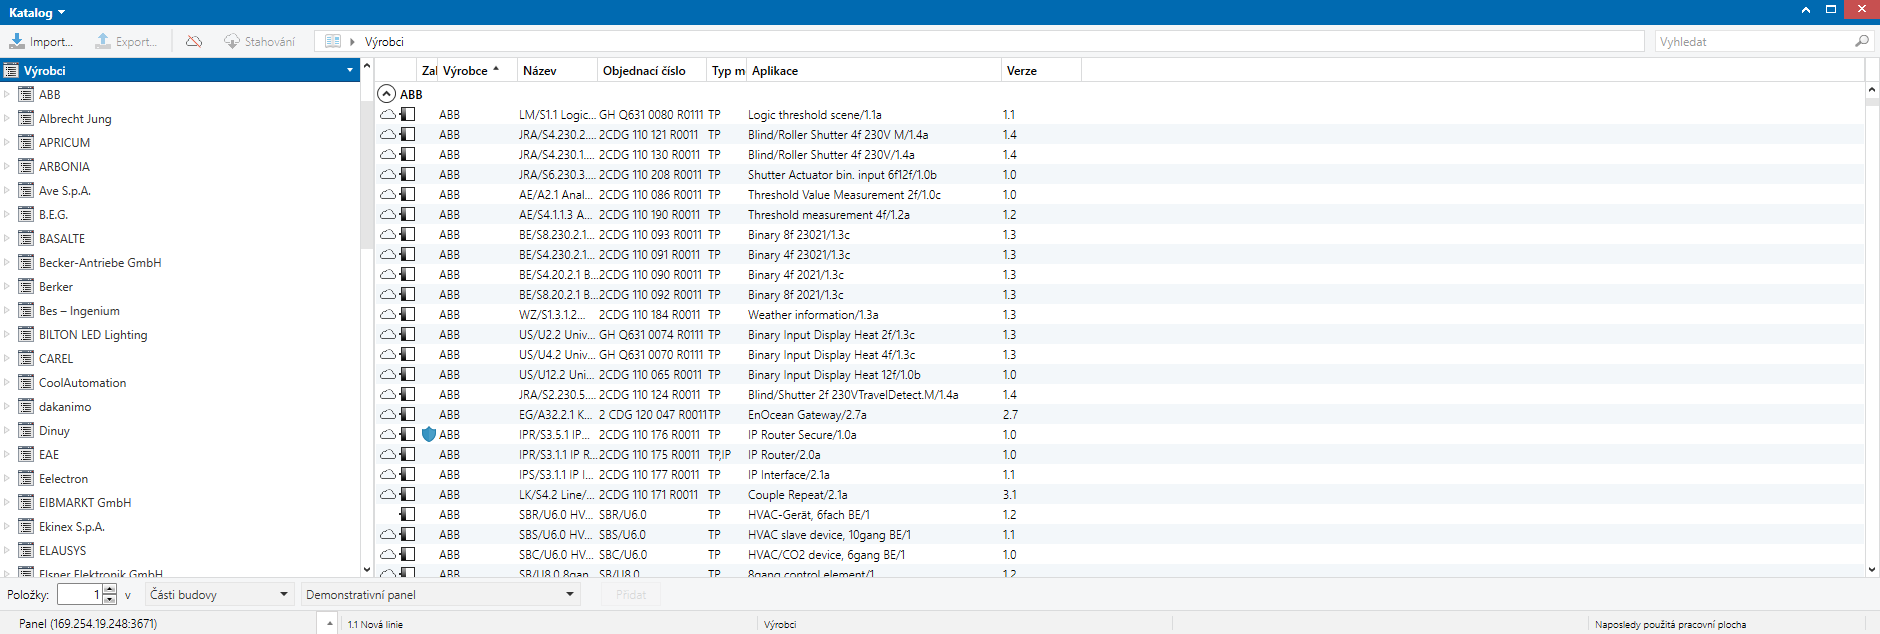
\includegraphics[width=1\columnwidth]{obrazky/Katalog.png}
				\caption{Katalog}
				%\caption{Popisek obrázku}%
				%\label{obr:ukazka}
			\end{figure}
\end{frame}


\begin{frame} 
	\frametitle{Tvorba instalace}
	
	\begin{columns}[T] 								% prostředí sloupce s umístěním nahoře
		\begin{column}{0.35\textwidth}		% první sloupec
			Pracovní plocha znázorňuje:\\[2ex]
			\begin{itemize}
				\item Umístění.
				\item Individuální adresy.
				\item Aplikační program.
				\item Výrobce.
				\item Produkt.
			\end{itemize}
		\end{column}
		%
		\begin{column}{0.75\textwidth}		% druhý sloupec
			\begin{figure}%	
				\centering
				\vspace{1cm}	              % horizontální mezera
				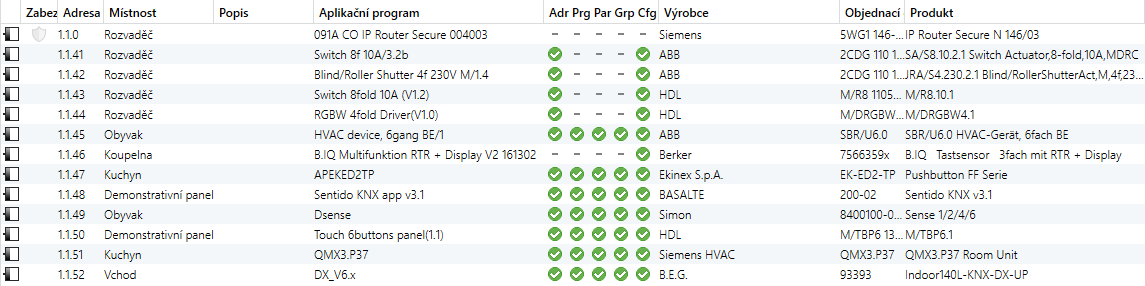
\includegraphics[width=1\columnwidth]{obrazky/Přístroje v ETS.png}
				\caption{Přístroje v ETS}
				%\caption{Popisek obrázku}%
				%\label{obr:ukazka}
			\end{figure}
		\end{column}
	\end{columns}											% ukončení prostředí sloupce
\end{frame}

\begin{frame} 
	\frametitle{Parametrizace}
	\begin{itemize}
	    \item Výběr provedení.
	    \item Nastavování vnitřních senzorů.
	    \item Nastavování funkcí.
	    \item Nastavování scén.
	\end{itemize}
			\begin{figure}%	
				\centering
				\vspace{0.2cm}	              % horizontální mezera
				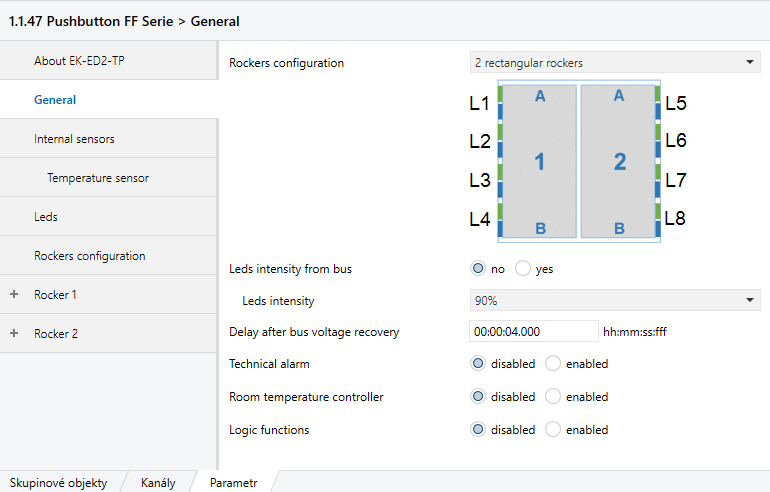
\includegraphics[width=.5\columnwidth]{obrazky/Ukazka parametrizace.png}
				\caption{Ukázka parametrizace}
				%\caption{Popisek obrázku}%
				%\label{obr:ukazka}
			\end{figure}
\end{frame}

\begin{frame} 
	\frametitle{Tvorba skupinových adres}
	\begin{itemize}
	    \item Kroky tvorby skupinových adres:	
	        \begin{itemize}
	            \item Vytvoření hlavní skupinové adresy.
	            \item Vytvoření střední skupinové adresy.
	            \item Vytvoření podskupinové adresy.
	            \item Vložení objektů z přístrojů.
	        \end{itemize}
	\end{itemize}

			\begin{figure}%	
				\centering
				\vspace{0.2cm}	              % horizontální mezera
				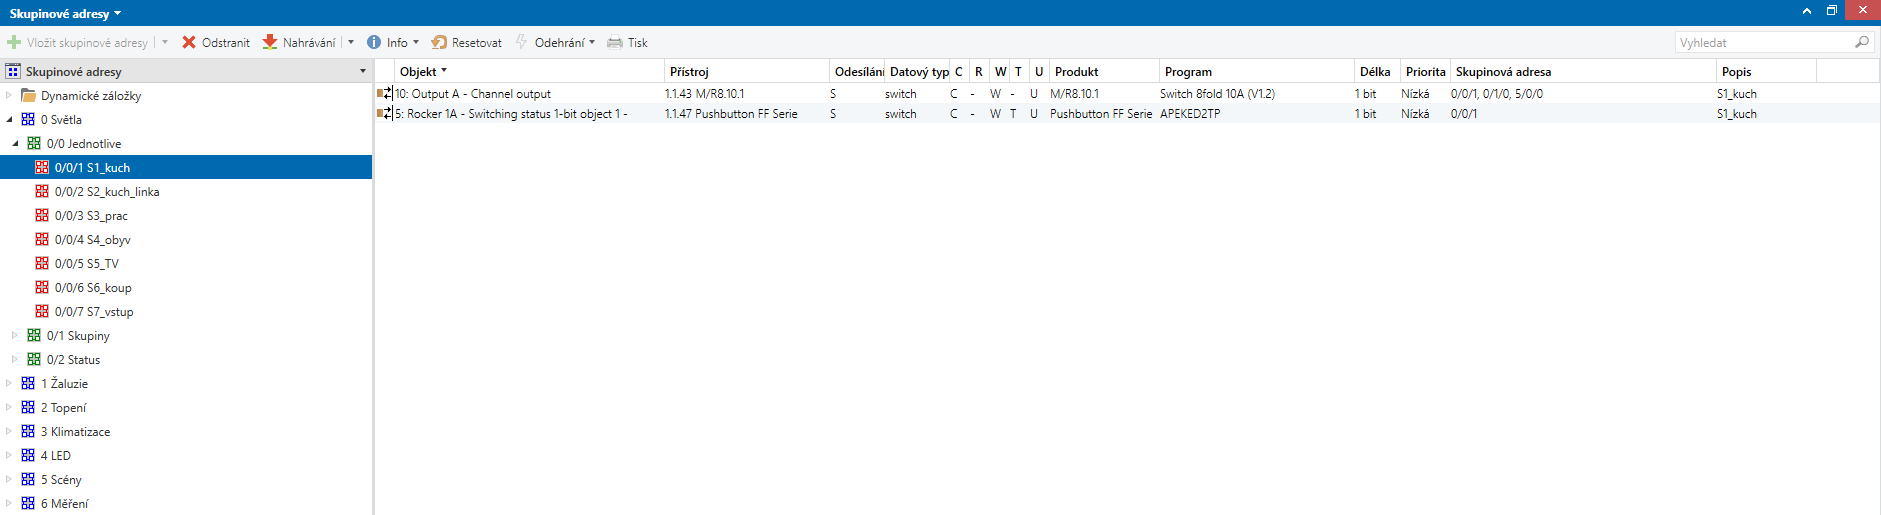
\includegraphics[width=1\columnwidth]{obrazky/Ukazka skupinovych adres.png}
				\caption{Ukázka skupinových adres}
				%\caption{Popisek obrázku}%
				%\label{obr:ukazka}
			\end{figure}
\end{frame}

%%%%%%%%%%%%%
\begin{frame} 
	\frametitle{Výsledky}
	\begin{columns}[T] 								% prostředí sloupce s umístěním nahoře
		\begin{column}{0.6\textwidth}		% první sloupec
	        \begin{itemize}
	            \item Hotová kapitola zaměřená na sběrnicový systém KNX.
	            \item Navázaný kontakt se společností Flowbox.
	            \item Hotová kapitola zaměřená na práci v ETS.
	            \item Funkční program.
	            \item Nenastavitelné tlačítko Berker.
	        \end{itemize}
	    \end{column}
	    
	\begin{column}{0.4\textwidth}		% druhý sloupec
			\begin{figure}%	
				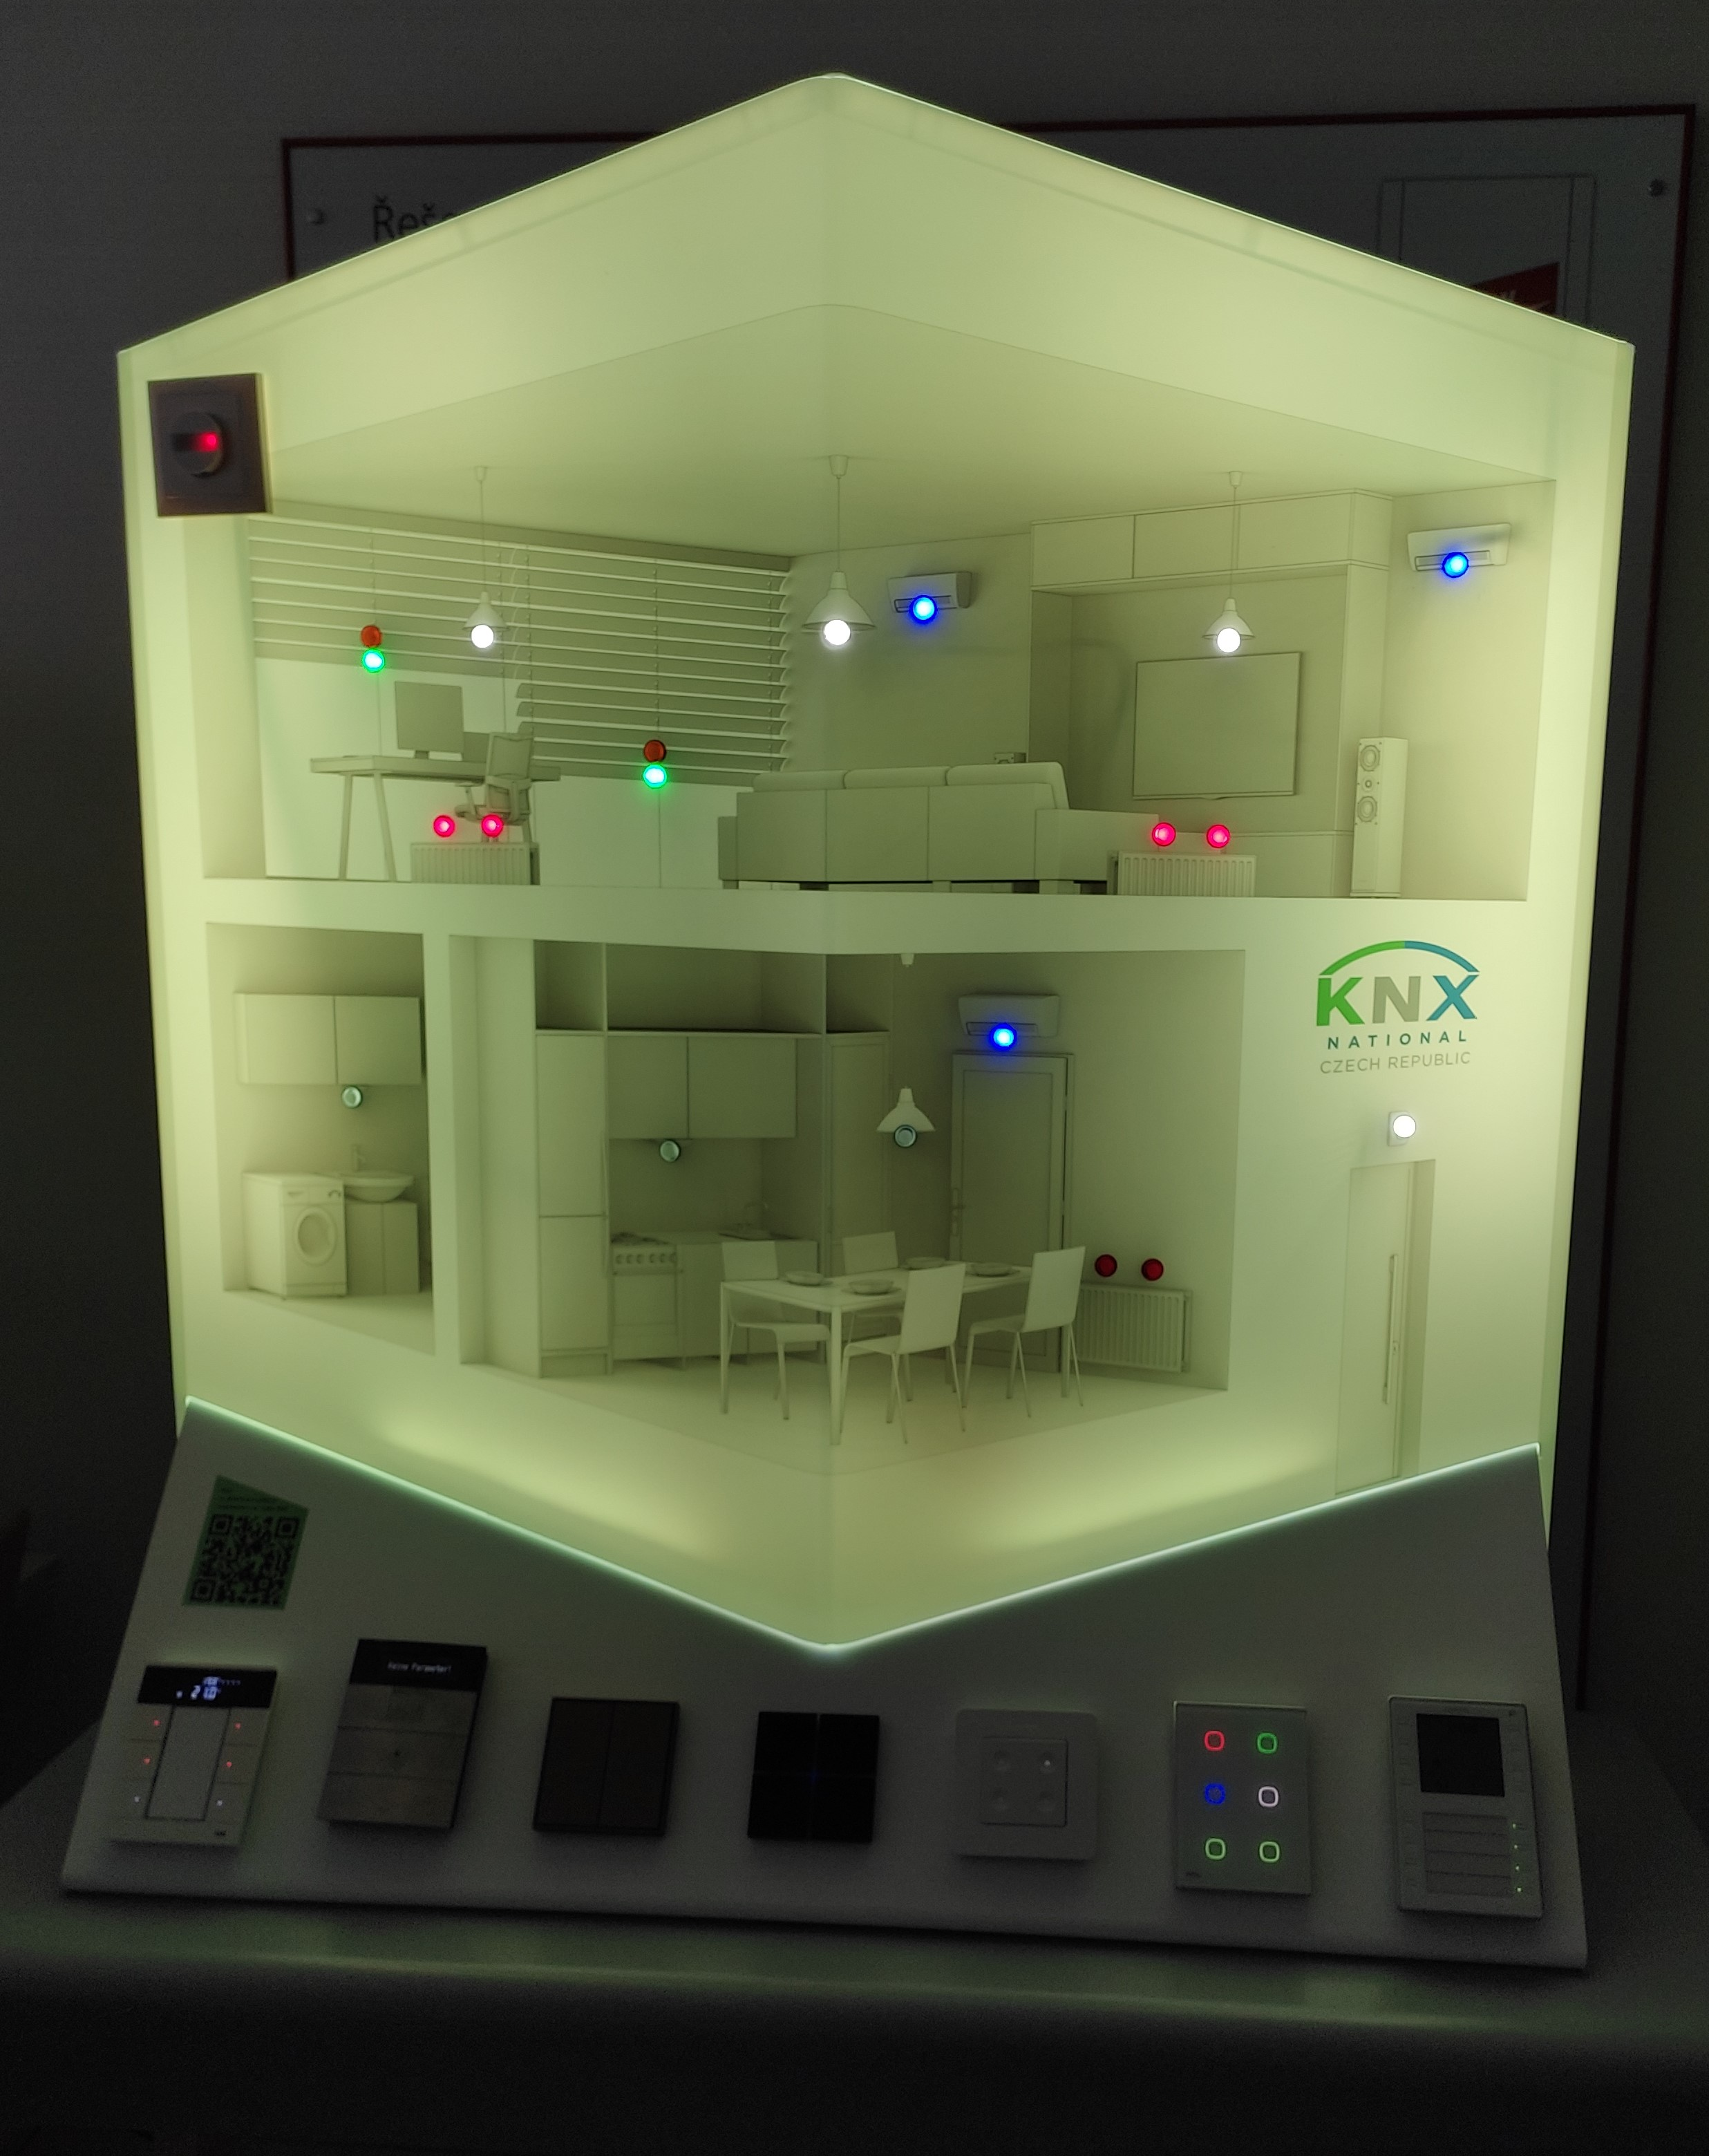
\includegraphics[width=.8\columnwidth]{obrazky/IMG_20211217_121402.jpg}
				\caption{Nastavený panel}
				%\caption{Popisek obrázku}%
				%\label{obr:ukazka}
			\end{figure}
		\end{column}
	\end{columns}
\end{frame}


%%%%%%%%%%%%%
\begin{frame} 
	\frametitle{Závěr}
\begin{itemize}
    \item Pro bližší seznámení s problematikou nutno absolvovat školení KNX.
    \item Více, než polovina práce je hotova.
    \item Do dalšího vydání práce:
        \begin{itemize}
            \item Nutnost změny dynamických scén.
            \item Vytvoření komunikačního driveru ve spolupráci se společností Flowbox.
            \item Vytvoření vizualizace skrze server Flowbox.
        \end{itemize}
\end{itemize}
\end{frame}


% podekovani
\begin{frame}[c] 
% bez nadpisu snímku
	\frametitle{\mbox{ }}
	\begin{center}
		{\Huge Děkuji za pozornost!}
	\end{center}
\end{frame}

% otázky oponenta
%\frame{
%\frametitle{Otázky oponenta}
%	\emph{Jaká je souvislost Vašeho vzorce (1.2) s~Maxwellovými rovnicemi v~integrálním tvaru?}\\[2ex]
	%
%	Již staří Římané\,\dots
%}

\end{document}

